% Desarrollo
% Sergio Cuellar
% 30 de abril 2011

\chapter{Proyectos desarrollados}
\label{chap:desarrollo}

A continuación se presentan algunas actividades desarrolladas en la empresa.

\section{Auditoría Electrónica}
\label{sec:auditoria}

La operación del negocio debe ser vigilada por algún medio, en el cual se plasme un historial de ventas de cada caja registradora en KFC. Es por esto que se cuenta con un impresor de tickets llamado de auditoría, el cual imprime el resumen de venta de cada ticket de cada caja.

Una de las necesidades de negocio más importantes es la de reducción en el costo de venta. Por lo que se tomó la decisión de eliminar este impresor y almacenar la auditoría de manera electrónica. Con esto se ahorra los impresores de tickets, los gastos en mantenimiento de éstos y los rollos de papel en los más de 230 restaurantes KFC.

Ambos modelos de cajas cuentan con puertos seriales para conectar impresores, además de poseer con un puerto Ethernet RJ-45. Cada caja registradora cuenta con una dirección IP privada para la comunicación con la caja \textit{master}, la cual se encarga, a través de este medio, de transmitirles programación y de recibir los tickets de las demás cajas, para formar la auditoría. 

Por lo que se puede observar de esta descripción, es que hay dos maneras posibles de capturar la auditoría de la caja master: por el puerto serial que manda los datos al impresor, o mediante la captura de los paquetes de red que le llegan a la caja master provenientes de las demás cajas. Se optó por usar la salida del puerto seria hacia al impresor, ya que al mandar a imprimir se manda el ticket integro junto con los caracteres de control para la impresora. De la otra manera, se hubiese tenido que estudiar el protocolo de envío de información de las cajas a la caja master; lo que se sabe de manera certera, es que la comunicación es tipo UDP\footnote{User Datagram Protocol}.

Al estar configurada la caja master para manejar la auditoría, se debe especificar el puerto serie por el que se mandará a imprimir, en caso de no tener conectado un impresor, la caja marcará un error en su pantalla. Eso significa que la caja se encuentra continuamente solicitando un status a la impresora.

El concentrador de puertos seriales es el modelo AccelePort  Xem de la marca Digi, el cual posee 8 puertos tipo RJ-45, con posibilidad de aumentar el número de módulos para poder soportar más dispositivos.

\begin{figure}[htb]
 \begin{center}
  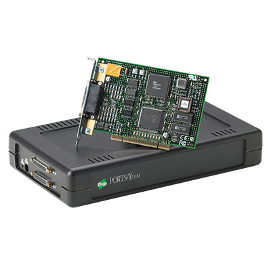
\includegraphics[scale=0.5]{acceleport_xem_lg.png}
 \end{center}
 \caption{AccelePort Xem de Digi con su tarjeta}
 \label{fig:digi}
\end{figure}

La configuración que indica el fabricante Digi para realizar un cable para impresora RJ-45 a DB-9 es el siguiente:


\begin{center}
 \resizebox{15cm}{!}{
  \begin{tabular}{|c|c|c|c|c|}
   \hline
   Pin RJ-45 & Señal & Dirección & Señal & Pin DB-9 \\
   \hline
   3 & GND (Tierra) & \textless\textendash\textgreater & GND (Tierra) & Carcaza \\
   \hline
   4 & TxD (Transmit Data) & \textendash\textgreater & RxD (Receive Data) & 2 \\
   \hline
   5 & RxD (Receive Data) & \textless\textendash & TxD (Transmit Data) & 3 \\
   \hline
   6 & SG (Signal Ground) & \textless\textendash\textgreater & SG (Signal Ground) & 5 \\
   \hline
   7 & CTS (Clear to Send) & \textless\textendash & DTR (Data Terminal Ready) & 4 \\
   \hline
   1 & DCD (Data Carrier Detect) & \textless\textendash & RTS (Request to Send) & 7 \\
   \hline
   2 & RTS (Request to Send) & \textendash\textgreater & CTS (Clear to Send) & 8 \\
   \hline
   8 & DTR (Data Terminal Ready) & \textendash\textgreater & DSR (Data Set Ready) & 6 \\
   \hline
  \end{tabular}
 }
\end{center}

Para poder saber qué datos manda la caja hice uso de un cable con el que se pueda leer la comunicación de la caja registradora (DB-9) al impresor de auditoría (DB-25). Por lo que abrí el cable e inserté las líneas descritas en la configuración anterior para un RJ-45, de esta manera se cuenta con un cable capaz de leer los datos mandados por la caja registradora. Para la lectura de estos datos utilice el software \textit{minicom}. Este es un programa de software libre utilizado para monitorear el puerto serie, análogo al \textit{Hyperterminal} de Windows. Los resultados indicaron que la caja manda el ticket con únicamente la información necesaria como número de productos, el producto, el costo del producto, el subtotal, el total, fecha, hora, número de ticket y el cajero que lo tomó. Además de estos datos, se cuentan con caracteres de control especiales para el impresor.

Otra característica que observé fue que la caja constantemente se comunica con el impresor para saber si está conectado y este último le manda una respuesta. Por lo que el programa desarrollado en C tendría que: limpiar los caracteres de control, y emular la comunicación que establece la caja registradora par evitar que marque error.

El cable original que va de la caja (DB-9) al impresor (DB-25) tiene la siguiente configuración:

\begin{center}
  \begin{tabular}{|c|c|c|c|}
   \hline
   Pin DB-9 & Señal DB-9 & Pin DB-25 & Señal DB-25 \\
   \hline
   1 &  DCD & 4 y 5 & RTS y CTS \\
   \hline
   2 & RxD & 2 & TxD \\
   \hline
   3 & TxD & 3 & RxD \\
   \hline
   4 & DTR & 6 y 22 & DSR y Ring indicator \\
   \hline
   5 & SG & 7 & SG \\
   \hline
   6 y 9 & Ring indicator y DSR & 20 & DTR \\
   \hline
   7 y 8 & CTS y RTS & 8 & DCT \\
   \hline
  \end{tabular}
\end{center}

De acuerdo a la configuración anterior y la indicada por el fabricante para el cable DB-9 a RJ-45, realicé la siguiente configuración de cable:

\begin{center}
 \begin{tabular}{|c|c|}
  \hline
  RJ-45 & DB-9 \\
  \hline
  1 & 7 y 8 \\
  \hline
  2 & 4 \\
  \hline
  3 & carcaza \\
  \hline
  4 & 2 \\
  \hline
  5 & 3 \\
  \hline
  6 & 5 \\
  \hline
  7 & 4 \\
  \hline
  8 & 6 \\
  \hline
 \end{tabular}
\end{center}

Desarrollé en lenguaje C el programa que lee los datos de la caja y además emula la respuesta del impresor a la caja. El programa \textit{portAudit} recibe como argumento el puerto serie del concentrador en el cual está conectado el cable. El programa \textit{portAudit} recibe como variable de ambiente el tipo de caja: \texttt{PORT\_TIPO\_CAJA=790} y \texttt{export PORT\_TIPO\_CAJA=5500} ya que los caracteres de control son distintos para cada caja registradora. Creé un script encargado de establecer estas variables, la configuración del puerto serial (velocidad, paridad, etc.) y la ejecución del binario.

El programa detecta la caja que originó el ticket, y de acuerdo a esta información la almacena en un archivo de texto para cada caja, además de un archivo que concentra la información de todas las cajas.

De acuerdo a la versión del sistema operativo en restaurantes, añadí una entrada en el archivo \texttt{/etc/inittab} para poder controlar de manera automática el inicio del servicio de almacenamiento de auditoría de manera automática de acuerdo al nivel de ejecución del sistema. 

A continuación se muestran dos tickets de ejemplo de auditoría:

\begin{Verbatim}[fontsize=\small]
    #335                 LLEV  
 4 MIXTA   
 1 PQ8BI SE                125.00  
   1 PAPFADO                35.00  
   1 NINGUNO                  .01  
           VTPR            160.00  
           TOTL       160.00  
           EFVO            200.00  
           CAMB             40.00  
NACHO  
  8377 10:51 #12 MAR.01'11  REG0003  
 


    #336                 COME  
 1 MBBIG C                  72.00  
   1 +PUR/RE                 7.00  
   1 NINGUNO                  .01  
 1 MANZANA   
           TOTL         79.00  
           EFVO            100.00  
           CAMB             21.00  
NACHO  
  8378 11:20 #12 MAR.01'11  REG0003  
\end{Verbatim}

Los tickets número 335 y 336 indican que provienen de la caja 3. El \#335 es un pedido para llevar y el \#336 es para comer en el restaurante. Se muestran las cantidades de los productos, su precio, el total, el efectivo con que se pagó y el cambio, el número de ticket único, así como la fecha y hora. El ticket \#335 que se manda a imprimir para dárselo al cliente se muestra a continuación:

\begin{Verbatim}[fontsize=\small]
 PREMIUM RESTAURANT BRANDS SDE RL DE CV  
     PASEO DE TAMARINDOS 400 PISO1       
   BOSQUES DE LAS LOMAS, CUAJIMALPA      
          MEXICO, D.F. 05120             
           RFC PRB100802H20              
--------------------------------------   
 #335       LLEV  
 4 MIXTA   
 1 PQ8BI SE                125.00  
 1 PAPFADO                  35.00  
 1 NINGUNO                   0.00  
          -------------------------  
           TOTAL A PAGAR     160.00  
Ciento Sesenta Pesos 00/100 M.N.  
           EFVO            200.00  
           CAMB             40.00  
                                         
      Sucursal KFC Div. del Norte        
      AV. DIVISION DEL NORTE 2855        
      PARQUE SAN ANDRES C.P.04040        
        MEXICO,DISTRITO FEDERAL          
NACHO  
  8377 10:51 #12 MAR.01'11  REG0003  
          No. ticket unico: 6     
    (solo se factura el mismo dia)       
         Gracias por su compra           
\end{Verbatim}

Para la verificación del correcto funcionamiento del \texttt{portAudit} creé un script que valida que todas las cajas estén registrando auditoría, y que no falte ningún ticket. Esto se realiza verificando primero, la existencia de la auditoría de las cajas en donde ya haya habido venta, después se busca el número de ticket en los archivos generados por la interfase que convierte la información de la caja registradora al punto de venta, y se revisa que en la auditoría correspondiente a la caja se encuentre. En caso de que no esté en ejecución el \texttt{portAudit}, que no se estén generando los archivos de auditoría o falten tickets de auditoría se genera un correo electrónico de manera automática para avisar de la situación correspondiente. Este script se ejecuta mediante CRON cada veinte minutos.

Ejemplo de correo electrónico cuando falta el archivo de auditoría de alguna caja:

\begin{Verbatim}[fontsize=\tiny]
Received: from xxxxxxxx.xxx.com.mx (192.168.101.xxx) by xxxxxxxx.xxx.com
 (xxx.xxx.xxx.xxx) with Microsoft SMTP Server id 14.0.639.21; Mon, 13 Jun 2011
 15:00:31 -0500
Received: from xxxx.xxx.com.mx (unknown [xx.xxx.xx.xxx])	by
 linuxeon.prb.com.mx (Postfix) with ESMTP id 07CCC2531;	Mon, 13 Jun 2011
 15:00:29 -0500 (CDT)
From: <mx0628r@xxx.com.mx>
To: <sergio.cuellar@xxx.com.mx>, <anibal.avelar@xxx.com.mx>,
	<jesus.noriega@xxx.com.mx>, <juanjose.martinez@xxx.com.mx>,
	<yaneth.yanez@xxx.com.mx>, <hugo.jacobo@xxx.com.mx>
Message-ID: <10776760.0.1307977209538.JavaMail.root@S062801>
Subject: Port de Auditoria CC 0628 13-06-2011-15:00: FALTA ARCHIVO DE ALGUNA
 CAJA
Content-Type: text/plain; charset="ISO-8859-1"
Content-Transfer-Encoding: 7bit
Date: Mon, 13 Jun 2011 15:00:29 -0500
Return-Path: mx0628r@xxx.com.mx
X-MS-Exchange-Organization-AuthSource: mexxch02.xxx.com
X-MS-Exchange-Organization-AuthAs: Anonymous
MIME-Version: 1.0

Falta(n) archivo(s) de auditoria de caja(s):
04


* Revisar banderas de cajas
* Revisar conexion de cables
* Revisar concentrador
\end{Verbatim}

El gerente del restaurante puede revisar los tickets de auditoría y del punto de venta mediante un reporte tipo web, en donde le indica la fecha que requiere consultar y como opción tiene la de ingresar el número de ticket a buscar, en caso de que no ingrese este dato, se despliegan todos los tickets del día. Esto se logra gracias a que los tickets de auditoría son almacenados en un directorio específico. El reporte consulta el archivo de acuerdo a la fecha seleccionada. 

\begin{figure}[htb]
 \begin{center}
  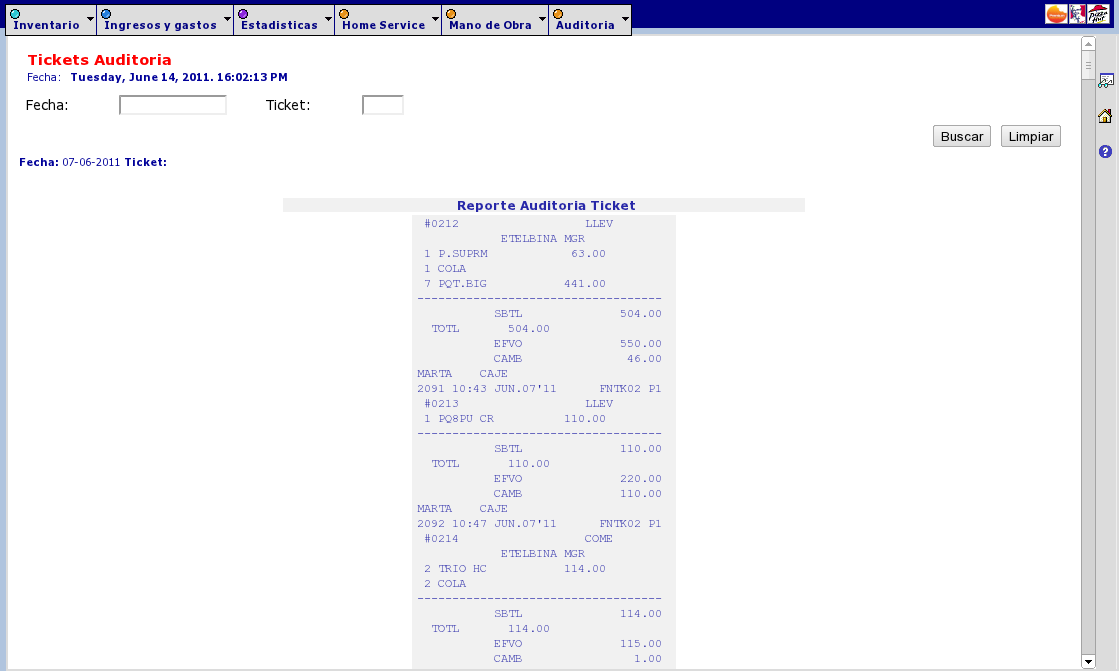
\includegraphics[scale=0.5]{ticket_audit_ereports.png}
 \end{center}
 \caption{Resultado de una consulta al reporte web de Ticket de Auditoría}
 \label{fig:rep_audit_ereports}
\end{figure}

Con esta solución se ha tenido un gran ahorro económico derivado de dejar de consumir papel, cintas de tinta, impresores y su mantenimiento. Igualmente se tiene un impacto benéfico a la ecología, ya que se deja de utilizar una cantidad importante de papel, teniendo una auditoría \textit{paperless}.

\section{Reporte de Estimado de Usos Ideales en KFC}
\label{sec:usos_ideales_kfc}

En KFC (y Pizza Hut) se necesita saber con anticipación el número de transacciones que se tendrán para cada día, de esta manera se puede saber, mediante un pronóstico, el número de hamburguesas que se deben preparar, el número de piezas de pollo que se deben marinar para posteriormente cocinarlas, el número de purés que se deben tener listos, etc. De esta manera la operación del restaurante está preparada para el nivel de transacciones que se tengan durante el día. Sabiendo esto, el gerente sabe el nivel de inventario que debe tener para satisfacer las transacciones, el número de piezas de pollo que debe descongelar, el número de asociados (empleados) que debe tener a cierta hora del día para poder preparar los productos, etc. 

El uso ideal es la cantidad de producto que el restaurante tuvo que haber usado, de acuerdo a su número de transacciones, y a la cantidad de producto establecida por la receta, sin incluir la merma. La merma son los productos, ingredientes o artículos que deben ser descartados debido a: deterioro, han expirado o se produjeron en exceso. La diferencia entre el uso ideal y el uso actual se le conoce como varianza, y puede ser expresada en cantidad de productos o en su valor monetario. Si la varianza es negativa significa que un producto o ingrediente fue utilizado más que la cantidad ideal; si es positiva, un producto o ingrediente fue utilizado menos que lo que dice el ideal.

El uso ideal se conoce una vez que han cerrado las ventas para el día y se generan los reportes del punto de venta. Para el gerente de restaurante es importante saber cuántos vasos, tapas, panes, kilos de papa debe tener listos para la operación de un día específico. Para esto debe conocer el pronóstico en el número de transacciones que tendrá para un día específico. No es lo mismo un domingo que un martes, ni un 16 de diciembre, que un 24 de diciembre. Una vez conocido el número de transacciones pronosticadas, el gerente, debe investigar cuál día tuvo ese número de transacciones, pero ahora reales. Una vez hecho esto debe consultar un reporte de esa fecha generado por el punto de venta donde se encuentran los usos ideales y obtener de el reporte el uso ideal de los productos que necesite.

Esto ocasiona que el gerente ocupe mucho tiempo en la búsqueda de estos usos ideales, por lo que desarrollé un reporte que automatice esta actividad.

Para facilitar la elaboración de este reporte, creé una tabla en la base de datos de PostgreSQL que almacene los usos ideales por fecha y por identificador de producto. Estos datos se obtiene de un comando que ya existe en el sistema y mediante un script en Perl se parsean los resultados y se ingresan a la base de datos. Esta carga se realiza de manera diaria, una vez que se han generado los usos ideales del día anterior. 

Esta es la descripción de la tabla de PostgreSQL encargada de almacenar los usos ideales:

\begin{Verbatim}[fontsize=\tiny]
    Table "public.op_inv_ideal_use"
  Column   |     Type      | Modifiers 
-----------+---------------+-----------
 turn_date | date          | not null
 turn_id   | smallint      | not null
 inv_id    | character(6)  | not null
 ideal_use | numeric(12,2) | 
 unit_cost | numeric(12,2) | 
 misc      | boolean       | 
Indexes:
    "op_invc_ideal_use_pkey" PRIMARY KEY, btree (turn_date, turn_id, inv_id)
Foreign-key constraints:
    "fk1" FOREIGN KEY (inv_id) REFERENCES op_grl_cat_inventory(inv_id) ON UPDATE RESTRICT ON DELETE RESTRICT
\end{Verbatim}

La llave foránea \texttt{inv\_id} pertenece a la tabla \texttt{op\_grl\_cat\_inventory}, la cual contiene, entre otros datos, el nombre del producto y la unidad de medida.

El los restaurantes existe una aplicación llamada \textit{e-Reports}\pageref{sec:ereports}, la cual está desarrollada en JSP\footnote{Java Server Pages}. En está aplicación se añaden los reportes requeridos clasificándolos de acuerdo a su finalidad. El reporte de ``Usos Ideales'' se  encuentra en el menú de \textit{Mano de Obra \textendash\textgreater Planeación \textendash\textgreater Usos Ideales Diarios}.

Creé archivos de configuración de productos clasificados de acuerdo a la línea de producción donde son utilizados. Los archivos son:

\begin{itemize}
 \item Biscuits.conf
 \item Ensalada.conf
 \item Marinado.conf
 \item Pure.conf
 \item Sandwich.conf
 \item Trasempaque.conf
 \item Congelados.conf  
 \item Home\_Delivery.conf
 \item Pure\_Ensalada.conf  
 \item Servicio.conf
\end{itemize}

En ellos se encuentra el número de inventario del producto a deplegar en el reporte. A continuación se muestra una parte del archivo de \texttt{Servicio.conf}:

\begin{Verbatim}[fontsize=\small]
#####################
###   Servicio    ###
#####################
# Caja regular
10519
# Tapa vaso 12 oz
10738
# Caja Economica
10517
# Servilletas
10570
# Tapa 32 oz
10830
# Bucket
10946
# caja chicky
10593
# Char porta vaso
10613
# Catsup sobre
10559
\end{Verbatim}

Teniendo estos archivos de configuración resulta muy fácil añadir o quitar productos de acuerdo a las necesidades de la operación.

El reporte obtiene de la tabla \texttt{op\_gt\_real\_sist\_mng} el pronóstico de número de transacciones y las transacciones reales más cercanas a la fecha seleccionada.

A continuación se muestra una pantalla de resultados del reporte:

\begin{figure}[htb]
 \begin{center}
  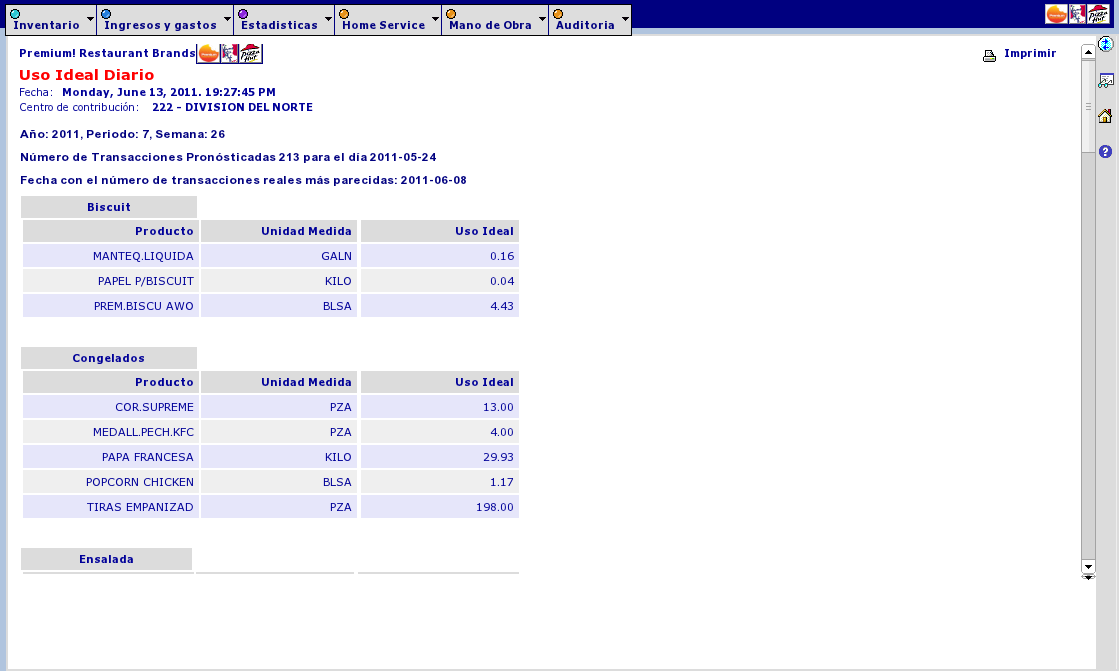
\includegraphics[scale=0.5]{ideal_use_2.png}
 \end{center}
 \caption{Usos Ideales Diarios en KFC}
 \label{fig:usos_ideales_kfc}
\end{figure}

\section{Cierre de Lote de Tarjeta de Crédito}
\label{sec:cierre_lote}

El uso de tarjetas de crédito y débito es indispensable para cualquier negocio ya que al no aceptarlas se pueden perder valiosas transacciones. Las tarjetas, hoy en día, no sólo son un método o forma de pago, sino que da seguridad a quienes la aportan, tanto seguridad al no portar efectivo como seguridad de poder pagar a largo plazo en caso de que no cuenten con el dinero, además de poder tener diferentes beneficios con sus puntos que otorga el banco al realizar compras, como viajes, artículos entre otros.

Actualmente la compañía ya cuenta con el servicio de cobro de tarjetas en la marca PH y se encuentra en un mercado prueba para la marca KFC, ambos obtuvieron excelentes resultados, tanto en transacciones como en un aumento en el ticket promedio por lo que se ha tomado la
decisión de realizar el lanzamiento nacional por fases hasta cubrir el 100\% de los restaurantes.

Existe una actividad muy importante que se debe realizar siempre al final del día, una vez que han concluido las ventas, el cierre de lote en las terminales bancarias. Con el cierre de lote se asegura que el banco depositará el dinero correspondiente a las ventas pagadas mediante tarjeta de crédito/débito, al siguiente día hábil. La importancia de esta actividad radica en las conciliaciones bancarias que se deben realizar de manera diaria, un retraso en el pago de este dinero ocasiona que no se puedan realizar a tiempo estas conciliaciones.

Por esta razón, la necesidad del negocio requiere de una aplicación en la cual los asociados ingresen el monto total cobrado de cada terminal bancaria, forzándolos ha haber realizado el cierre de lote en cada dispositivo. La aplicación fue desarrollada para \textit{e-Reports}.

Los únicos asociados autorizados para realizar el cierre de lote, son aquellos que poseen un nivel de seguridad 1 en el sistema de punto de venta. Creé una tabla en la base de datos de PostgreSQL (\texttt{ss\_cat\_terminals\_ccard}) que contiene información relacionada al número de terminales bancarias con el que cuenta el restaurante. De esta manera, únicamente se despliegan el número de terminales bancarias con las que cuente el restaurante.

Los datos que deben ser ingresados por cada terminal bancaria son:

\begin{itemize}
 \item Monto que indica el cierre de lote de la terminal. En caso de no haber cobrado con una terminal se debe ingresar \texttt{0.0}.
 \item Fecha en que se realiza el cierre de lote.
 \item Hora en que se realiza el cierre de lote.
 \item Número de transacciones que reporta la terminal.
 \item El campo de ``Cierre Fallido`` se utiliza en caso de que haya existido un error en la terminal bancaria, por ejemplo, por problemas de comunicación.
\end{itemize}

Una vez ingresados estos datos, se debe presionar el botón de \texttt{Obtener montos totales}, con esta acción, se obtiene la cantidad total de dinero registrado en las terminales bancarias y el total de ventas cobradas con tarjeta de crédito/débito que se tienen registrados en el sistema punto de venta. Estos totales, deben coincidir, en caso de no hacerlo, se muestra un mensaje indicando la diferencia y sugiriendo revisar los datos, y si es el caso, corregirlos. Después se debe presionar el botón de \texttt{Guardar y confirmar datos}, en esta parte es cuando se le solicita al asociado, elegir su nombre de usuario y teclear su contraseña. Una vez realizado esto de manera correcta se almacenarán los datos ingresados y en caso de haber exisitido diferencia entre los montos totales del sistema punto de venta y el de las terminales bancarias se manda un correo electrónico automático al restaurante, al gerente de zona y a las personas del área de Ingresos correspondientes.


\begin{figure}[htb]
 \begin{center}
  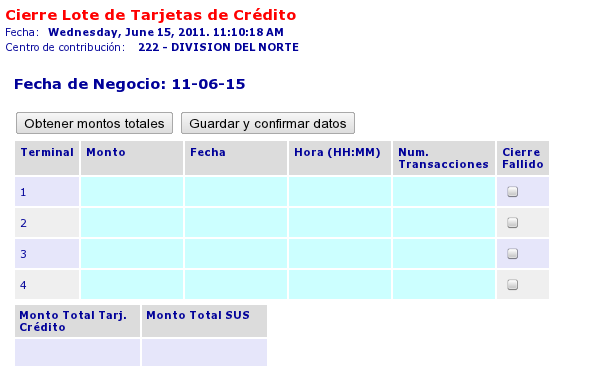
\includegraphics[scale=0.7]{cierre_lote_1.png}
 \end{center}
 \caption{Cierre de Lote de Tarjeta de Crédito en e-Reports}
 \label{fig:cierre_lote_1}
\end{figure}

Existe además, una alarma que funciona a manera de recordatorio, en caso de que no se haya realizado el cierre de lote a las 23:45 horas. La alarma, realizada en Perl y Xdialog, consiste en una ventana que aparece en la computadora del restaurante recordando ingresar los datos del cierre de lote, así como también la generación de \textit{beeps} en la misma computadora, y en caso de ser restaurante PH, en todas las terminales. Al desactivar la alarma, ésta solicitará por el usuario y contraseña de quien lo está realizando, esto con el fin de almacenar esta información en un archivo. En caso de que nadie la desactive, ésta automáticamente se apaga después de 15 minutos.

\begin{figure}[htb]
 \begin{center}
  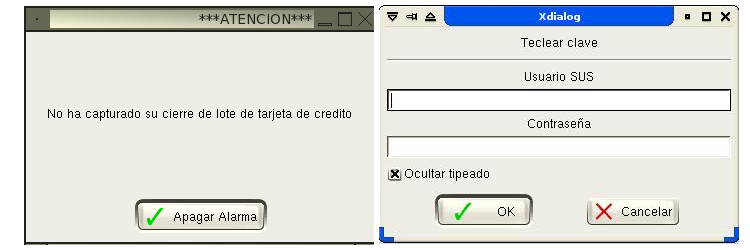
\includegraphics[scale=0.7]{cierre_lote_4.png}
 \end{center}
 \caption{Ventanas de Xdialog de la alarma}
 \label{fig:cierre_lote_4}
\end{figure}

Cada cierre de lote realizado en \textit{e-Reports} es almacenado en un archivo, con lo cual se puede tener un registro de este reporte. A continuación se muestra un ejemplo de archivo almacenado:

\begin{Verbatim}[fontsize=\small]
222|1|11-05-14|11-05-14|20:52|4874.20|5190.2|5190.2|0.0|28|SENI|14-5-2011 21:16:13
222|2|11-05-14|11-05-14|21:10|316|5190.2|5190.2|0.0|1|SENI|14-5-2011 21:16:13
222|3|11-05-14|11-05-14|00:00|0|5190.2|5190.2|0.0|0|SENI|14-5-2011 21:16:13
222|4|11-05-14|11-05-14|00:00|0|5190.2|5190.2|0.0|0|SENI|14-5-2011 21:16:13
\end{Verbatim}

Los campos indican:

\begin{description}
 \item[Primer campo] es el número del restaurante.
 \item[Segundo campo] es el número de terminal bancaria.
 \item[Tercer campo] es la fecha en la que se capturó el cierre de lote.
 \item[Cuarto campo] es la fecha negocio, la cual es la fecha que tiene el sistema punto de venta. En algunos casos puede que no coincida la fecha actual con la fecha de negocio.
 \item[Quinto campo] es la hora que marca la terminal bancaria al momento de realizar el cierre de lote.
 \item[Sexto campo] es el monto cobrado en la terminal bancaria.
 \item[Séptimo campo] es el monto total cobrado de las terminales bancarias.
 \item[Octavo campo] es el monto total que reporta el sistema punto de venta que fue pagado con tarjeta de crédito/débito.
 \item[Noveno campo] es la diferencia entre el monto total que reporta el sistema punto de venta y monto total cobrado de las terminales bancarias.
 \item[Décimo campo] es el número de transacciones cobradas en la respectiva terminal bancaria.
 \item[Onceavo campo] es el nombre de usuario que realizó el cierre de lote.
 \item[Doceavo campo] es el timestamp del sistema al momento de realizar el cierre de lote.
\end{description}


\section{Proyecto de Control de Asistencia mediante Lector de Huellas Digitales}
\label{sec:fingerprint}

La tecnología de lectores de huellas digitales está siendo usada en una gran variedad de aplicaciones e industrias. Provee mayor seguridad y evita el mantenimiento de contraseñas. La situación actual del negocio es que las personas en los restaurantes poseen una contraseña con la cual registran su entrada, la cual les permiten comenzar a realizar operaciones el sistema punto de venta,  y salida. Las horas trabajadas son tomadas en cuenta para el cálculo de la nómina. Las contraseñas pueden ser compartidas, dando lugar a que algún compañero realice las entradas de los demás, aún cuando éstos lleguen tarde. Así mismo la salida es un problema, ya es muy común que los empleados olviden realizar su salida, y el gerente puede ingresar sus horas de salida, lo que conlleva a malentendidos. Toda esta situación afecta directamente a la nómina, ya que no se están contando de manera real las horas trabajadas.

La oportunidad de negocio consiste en poder tener la certeza de que la persona que realiza la entrada/salida es realmente ella y que no hay posibilidad de suplantar a esta persona, con lo que se tendrían ahorros significativos en gastos de nómina. Además evitar las contraseñas para usar el sistema punto de venta implica una mayor seguridad y responsabilidad en las transacciones realizadas en él.

Las huellas digitales se pueden considerar como una tarjeta de identidad visible que la naturaleza nos dio. Éstas poseen un diseño único que representan únicamente a una persona. Las huellas digitales son diminutas arrugas en la piel de nuestros dedos, tanto de las manos como de los pies, las cuales resultaron de la evolución de nuestros ancestros y cuya finalidad es la de poder sujetar de mejor manera objetos. Además sirven para poder transmitir mejor las vibraciones lo que ocasiona que se puedan distinguir las características de las superficies.

Las huellas digitales se forman de acuerdo a una combinación de la carga genética del individuo y los factores ambientales en los cuales se desarrolla, por lo que es casi imposible que el patrón de una huella digital se repita. Como consecuencia, las huellas digitales son únicas en cada individuo, incluso en gemelos. Dos huellas digitales pueden parecer iguales a simple vista, pero si se observan con más cuidado, ya sea por un investigador entrenado o un software especializado, éstos pueden encontrar las diferencias. Se les llama \textit{minutias} a las características principales de una huella digital, con las que se pueden realizar comparaciones con otras huellas. Ejemplos de minutias son, que si una arruga tiene forma de Y, de U, el abrupto final de una arruga, etc. Las minutias son los patrones que se buscan y analizan en los programas especializados en reconocimiento de huellas digitales.

\begin{figure}[htb]
 \begin{center}
  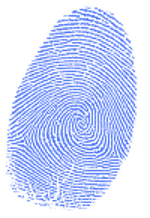
\includegraphics[scale=0.5]{fingerprint.png}
 \end{center}
 \caption{Huella Digital}
 \label{fig:finger_print_1}
\end{figure}


\subsection{Tipos de sensores}
\label{sec:fp_sensores}


Existen tres tipos de sensores (\textit{scanners}) de huellas digitales: ultrasónicos, ópticos y capacitivos, de los cuales los más comunes son los últimos dos.

Los scanners de huellas digitales involucran la captura de una imagen digital de la huella usando luz visible. Este tipo de sensor es en esencia una cámara digital. La capa superior del sensor, donde el dedo es colocado, se conoce como la superficie de contacto. Debajo de esta capa existe una capa que ilumina la superficie del dedo. La luz reflejada del dedo llega a un dispositivo de carga acoplada (\textit{CCD, charge-coupled device)} que captura la imagen de la huella digital. Una superficie de contacto sucia o rayada ocasiona una mala imagen de la huella digital.

Los scanners capacitivos, al igual que los ópticos, generan una imagen de la huella digital, pero en lugar de capturar la imagen mediante luz, se utiliza el principio de capacitancia. El sensor que contiene arreglos de pixeles funciona como una placa de un capacitor, la  capa de la piel, conocida como dermis (que conduce electricidad) es la otra placa, y la epidermis funciona como un dieléctrico.

\subsection{Ventajas y desventajas}
\label{sec:fp_pros_cons}

Existen diferentes maneras en las cuales un sistema de seguridad puede verificar que alguien es un usuario autorizado. La mayoría de los sistemas buscan por una o más de las siguientes sentencias:

\begin{itemize}
 \item Qué se tiene.
 \item Qué se sabe.
 \item Quién es.
\end{itemize}

Para entrar a un sistema tipo ''qué se tiene``, se necesita algún dispositivo como un token de autenticación, o una tarjeta RFID\footnote{Radio Frequency Identification}. Para el sistema ''qué se sabe`` se requiere que se ingrese una contraseña o un PIN. El sistema ''quién es`` busca por evidencia física de que la persona que se dice ser, es realmente ella, en esta clasificación entran las huellas digitales y el reconocimiento de voz.

Estos últimos sistemas tienen varias ventajas sobre los demás, por ejemplo:

\begin{itemize}
 \item Los atributos físicos son más difíciles de falsificar que las tarjetas de identificación.
 \item No se puede usar la fuerza bruta para adivinar una huella digital como se hace con las contraseñas.
 \item No se pueden olvidar las huellas digitales como sucede con una contraseña.
\end{itemize}

A pesar de ser tan efectivas, no son infalibles, y también tienen desventajas. Los scanners ópticos no siempre pueden distinguir bien entre la imagen de una huella digital, y una huella digital real. Y los scanners capacitivos pueden ser engañados con el molde de una huella digital. En uno de los peores casos, un criminal pudo haber cortado el dedo de una persona para poder acceder al sistema. Es por esto que algunos dispositivos ya cuentan con sensores de calor y pulso para poder distinguir estos casos.

Para hacer estos sistemas más robustos, conviene utilizar el análisis biométrico con un sistema convencional de identificación, como una contraseña. La necesidad del negocio no la requiere directamente, solamente como medio de respaldo en caso de que el dispositivo lector falle.

\subsection{Prototipo 1: Lector Microsoft}
\label{sec:lector_microsoft}

Al comenzar a realizar el proyecto se contaba con un lector de huellas digitales modelo ''Microsoft Fingerprint Reader``, el cual es un lector con conexión USB. La desventaja en un principio radicaba en la incertidumbre de que el dispositivo funcionara en una computadora con GNU/Linux. Al conectarlo y ejecutar el comando \texttt{dmesg} se observa que el kernel identifica correctamente el lector.

\begin{figure}[htb]
 \begin{center}
  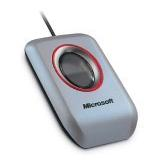
\includegraphics[scale=0.5]{microsoft_scanner.png}
 \end{center}
 \caption{Microsoft Fingerprint Reader}
 \label{fig:finger_print_2}
\end{figure}

Este lector está basado en un chipset conocido como \textit{DigitalPersona U.are.U 4000/4000B} el cual es usado en una gran cantidad de lectores, incluidos los de la compañía fabricante \textit{DigitalPersona}. El lector es del tipo óptico, el cual únicamente captura imágenes y los envía a la computadora y es necesario el uso de software para procesar y comparar las huellas digitales. Además el sensor es capaz de detectar cuando un dedo ha sido colocado o removido y se le puede indicar cuando capturar la huella digital.

Haciendo una investigación se encuentra que existe software libre que permite la lectura y procesamiento de las huellas digitales en GNU/Linux. Este software se llama \texttt{libfprint\footnote{http://www.freedesktop.org/wiki/Software/fprint/libfprint}}.  \texttt{libfprint} es una biblioteca que permite a los desarrolladores añadir soporte de lectores de huellas digitales a sus desarrollo. Algunas de sus características son:

\begin{itemize}
 \item Está escrito en lenguaje C.
 \item Depende de la biblioteca \texttt{libusb} y \textit{glib} para la comunicación.
 \item Ofrece una única interfaz de programación para la gran variedad de dispositivos que soporta.
 \item Soporta la captura y descarga en de imágenes en tiempo real desde el lector.
 \item Incluye funciones de procesamiento de imágenes.
 \item Permite el registro de huellas digitales de una persona (enrolamiento) y su verificación.
\end{itemize}

Los controladores propietarios de \textit{DigitalPersona} y su kit de desarrollo de software (SDK\footnote{Software Development Kit}) envían las imágenes cifradas a través de USB. Debido a que el método de cifrado es desconocido,  \texttt{libfprint} envía las imágenes sin esta protección.

\begin{figure}[htb]
 \begin{center}
  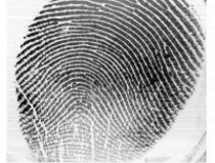
\includegraphics[scale=0.5]{fingerprint_raw_scan.png}
 \end{center}
 \caption{Ejemplo de imagen capturada por el dispositivo}
 \label{fig:finger_print_3}
\end{figure}

El lector manda una imagen de 348x289 píxeles separadas en dos transacciones, la primera es un encabezado de 64 bytes que es ignorada y después la imagen.

Uno de los grandes problemas con el sistema actual, es que a pesar de que funciona para lo que necesita hacer: tomar venta, generar reportes, etc., el sistema está sumamente desactualizado, por lo que la instalación de nuevo software puede conllevar a la actualización o instalación de nuevo software. Para la compilación del código fuente de \texttt{libfprint} se tuvo que instalar el siguiente software:

\begin{itemize}
 \item \textit{GLib} (ver. 2.28.0). Es una biblioteca de propósito general, originalmente parte de GTK+, pero a partir de la versión 2.0 los desarrolladores decidieron separarlas para crear un nuevo producto. GLib proporciona estructuras de datos avanzadas, como listas doblemente ligadas, tablas hash, arreglos dinámicos, árboles binarios, etc. Además provee de funciones para programación de hilos, colas, acceso seguro a memoria, timers, etc.
 \item \textit{ImageMagick} (ver. 6.6.0-4). Es una aplicación que sirve para crear, editar y componer imágenes. Puede leer, convertir y guardar imágenes en una gran variedad de formatos.
 \item \textit{libusb} (ver 1.0.8). Es una biblioteca que proporciona las funciones necesarias para el control en la transmisión y recepción de datos de un dispositivo USB.
 \item \textit{nss}. \textit{Network Security Services} es un conjunto de bibliotecas diseñadas por Mozilla para desarrollo de aplicaciones seguras cliente/servidor. Proporciona bibliotecas seguras como SSL\footnote{Secure Socket Layer} y S/MIME\footnote{Secure/Multipurpose Internet Mail Extensions}. Esta herramienta fue la más difícil de compilar y adaptar para el sistema actual, ya que tuve que adecuar algunos archivos del código fuente para que pudiese compilar. Además de que el código fuente que proporciona Mozilla no sigue un estándar (archivos \texttt{configure}, \texttt{Makefile} y \texttt{autoconf}) y su documentación es deficiente.
\end{itemize} 

Originalmente \texttt{libfprint} no es multiusuario, el software está diseñado para almacenar la información de las huellas digitales en el \texttt{\$HOME} de cada usuario, por lo que es necesario que los usuarios tengan una cuenta en el sistema. Para corregir este problema modifiqué el código fuente de \texttt{libfprint} con el objetivo de que se almacene la información de todos los usuarios en un solo directorio y en subdirectorios de acuerdo al número de empleado registrado en el punto de venta.

Desarrollé una interfaz gráfica usando \textit{Swing} para la entrada/salida y enrolamiento de los empleados. \textit{Swing} es una biblioteca gráfica para Java. Incluye widgets para interfaz gráfica de usuario tales como cajas de texto, botones, desplegables y tablas.

Debido a que \texttt{libfprint} está programado en C y la interfaz gráfica es en Java, utilicé JNI (\textit{Java Native Interface} para funcionar. \textit{JNI} es un framework de programación que permite que un programa escrito en Java ejecutado en la máquina virtual java (JVM) pueda interactuar con programas escritos en otros lenguajes como C, C++ y ensamblador, la desventaja más importante es la pérdida de portabilidad que ofrece Java.

Programé dos funciones en C usando JNI: la de verificación y la de enrolamiento. A continuación se muestra el encabezado del archivo de verificación:

\begin{Verbatim}
JNIEXPORT jint JNICALL Java_PRBAS_PRBAttendance_verify
  (JNIEnv *env, jobject obj, jint finger, jstring p, jstring u)
\end{Verbatim}

El apuntador \texttt{JNIEnv *env}, junto con \texttt{jobject obj} siempre deben ir al programar con JNI, ya que son interfaz con la máquina virtual de Java, después pueden ir los argumentos necesarios para la función, en este caso, \texttt{finger} que es un entero y representa al dedo a ser verificado (0-pulgar izquierdo, 1-índice izquierdo, 2-medio izquierdo, ... 9-meñique derecho), la cadena \texttt{p} indica la ruta donde se encuentra almacenada la información de las huellas digitales, y \texttt{u} es el usuario a verificar.

Una de las partes más importantes es poder ingresar al sistema punto de venta la información de entrada/salida de un empleado. No se tenía documentado exactamente cómo y dónde es que el sistema ingresa está información, por lo que tuve que revisar el código fuente para conocerlo. Para ingresar la entrada/salida el empleado debe teclear su clave en el sistema y posteriormente ingresar a las opciones de \textit{b) Entrada de Empleado} o \textit{c) Salida de Empleado}.

\begin{figure}[htb]
 \begin{center}
  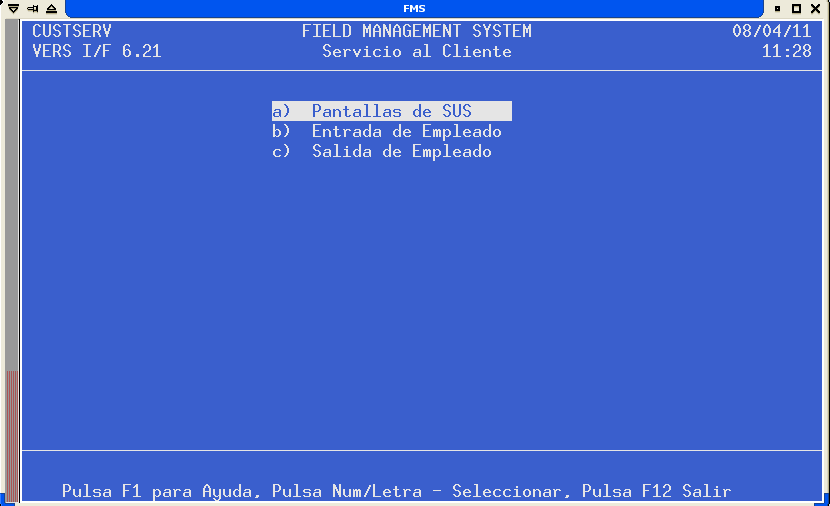
\includegraphics[scale=0.5]{fp_libfprint_fms_1.png}
 \end{center}
 \caption{Pantalla de entrada/salida en sistema punto de venta.}
 \label{fig:finger_print_4}
\end{figure}

Al realizar la entrada/salida el sistema utiliza los siguientes archivos binarios: 

\begin{enumerate}
 \item \texttt{/usr/fms/data/hrcempl.dat}
 \item \texttt{/usr/fms/data/tkeclk.dat}
 \item \texttt{/usr/fms/data/tkpaytrn.dat}
\end{enumerate}


El primero contiene los datos de todos los empleados, una línea por cada empleado: nombre, apellido, edad, dirección, etc. El siguiente archivo únicamente sirve para saber si un usuario ya registro su entrada, y contiene una copia de la línea correspondiente del archivo antes mencionado por cada usuario registrado. Y el último archivo contiene una línea por cada operación realizada de entrada y salida, identificadas con \texttt{TI} para entrada y \texttt{TO} para la salida.

El sistema punto de venta se utiliza principalmente mediante una interfaz gráfica, pero ésta se encuentra soportada por una gran cantidad de comandos que se pueden ejecutar en el shell; entre todos estos comandos, existe el comando\\ \texttt{/usr/fms/etc/sysdd} que sirve para poder poder convertir un archivo binario a texto plano, y viceversa, siempre y cuando se sepa la estructura del archivo binario. Por ejemplo, a continuación se muestra una parte de la estructura del archivo \texttt{/usr/fms/data/tkpaytrn.dat}:

\begin{Verbatim}
typedef struct  tkpaytrn_rec
{
    long    date;
    short   tran_group;
    char    fill1[2];
    char    emp_ssn[16];
    char    source;
    char    trancode[3];
\end{Verbatim}

El comando \texttt{/usr/fms/etc/sysdd} recibe de argumentos la operación a ejecutar, convertir de binario a texto es \texttt{btoa} y al contrario es \texttt{atob}. Después la estructura del archivo y al final el archivo, para este caso sería: 

\texttt{/usr/fms/etc/sysdd btoa lhs2s16cs3 /usr/fms/data/tkpaytrn.dat}

La \texttt{l} es para el tipo de dato \texttt{long}, la \texttt{h} para \texttt{short}, la \texttt{s} para arreglos \texttt{char} seguido por el número de elementos y \texttt{c} para un sólo \texttt{char}.

\begin{figure}[htb]
 \begin{center}
  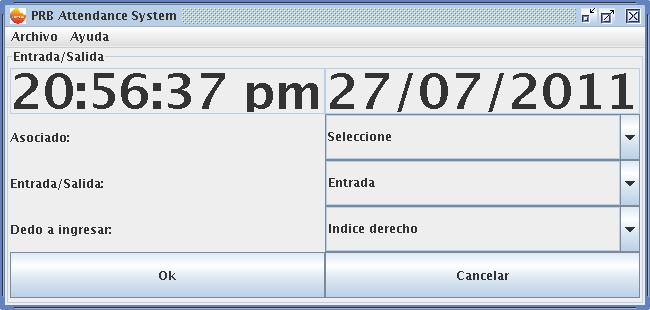
\includegraphics[scale=0.4]{fp_libfprint_attendance_1.png}
 \end{center}
 \caption{Pantalla de entrada/salida con lector de huellas digitales.}
 \label{fig:finger_print_5}
\end{figure}


En la figura \ref{fig:finger_print_5} se observa la interfaz en Swing de la aplicación de Entrada/Salida. Como se puede observar, ésta cuenta con la fecha y hora actual, con la cual se almacenará el registro. Al seleccionar el asociado se muestra una lista de todos los empleados registrados en el sistema punto de venta, los cuales son extraídos a través de comandos de SUS.

\begin{figure}[htb]
 \begin{center}
  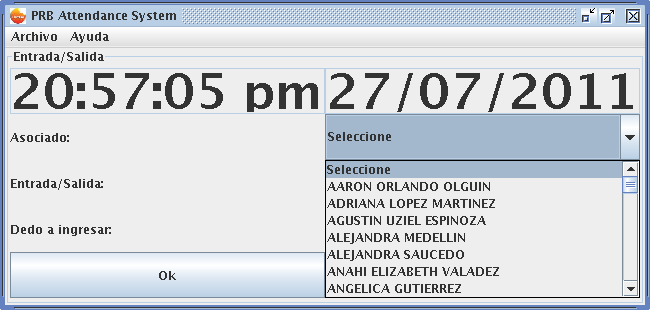
\includegraphics[scale=0.4]{fp_libfprint_attendance_2.png}
 \end{center}
 \caption{Listado de asociados.}
 \label{fig:finger_print_6}
\end{figure}

La selección de entrada/salida sirve para ingresar \texttt{TI} o \texttt{TO} en el archivo correspondiente. Un área de oportunidad en el desarrollo es la detección automática si es entrada o salida. Lo que sí debe ser seleccionado, debido a la naturaleza de la biblioteca \texttt{libfprint}, es la selección del dedo de la huella digital a ingresar. Esto se debe a que el software no es capaz de realizar la comparación entre todas las huellas digitales almacenadas de un mismo usuario, y mucho menos de realizar esta comparación para las huellas de todos los usuarios. Por lo que se le debe decir el usuario y el dedo a ingresar, para que el software únicamente haga la comparación de la huella a verificar y la que fue previamente almacenada. Al dar click en \texttt{OK}, se solicita al usuario que coloque el dedo correspondiente en el lector de huellas digitales, se recomienda colocarlo por alrededor de 3 segundos y retirarlo; el lector, como se mencionó anteriormente, es capaz de detectar la colocación  y remoción de un dedo. En caso de que no se haya verificado la huella digital, la interfaz solicitará que se vuelva a colocar el dedo. Esta interfaz aparece una vez que el usuario ha seleccionado la opción correspondiente (\texttt{b)} o \texttt{c)} de la figura \ref{fig:finger_print_4}).

Para el almacenamiento de las huellas digitales o el enrolamiento, se utiliza una interfaz más simple, en la cual únicamente se selecciona el usuario y el dedo. El procedimiento al hacer click en \texttt{OK} es el mismo que en la verificación. Por razones de seguridad y de evitar el múltiple enrolamiento de una misma huella digital para diferentes usuarios, esta funcionalidad se activa a petición del gerente del restaurante.

Es importante mencionar, que la biblioteca \texttt{libfprint} es capaz de obtener una fotografía de la huella digital, ésta no es utilizada para el análisis de las minutias, \texttt{libfprint} genera un archivo de datos binarios, el cual no puede ser leído por un editor de textos. La imagen de la huella digital es eliminada, ya que de acuerdo a la nueva \textit{Ley de Protección de Datos Personales en Posesión de los Particulares} se debe tener un mayor cuidado en el manejo en este tipo de datos para no caer en problemas legales.

Es por esto que busqué un dispositivo más especializado, el cual se describe con más detalle en la sección \ref{sec:lector_zksoftware}.

En las pruebas realizadas en este dispositivo observé que la verificación exitosa depende de la forma en que se haya capturado la huella digital en el enrolamiento. Debido a que el software únicamente usa una sola huella digital para obtener las minutias, al colocar de otra forma el dedo, ocasiona que muchas minutias no correspondan y arroje como resultado que la huella digital no corresponde. Esto ocasionaría un enorme problema en los restaurantes, elevando el número de soportes técnicos diariamente debido a que los empleados no pueden registrar su entrada ni entrar al sistema.

\subsection{Prototipo 2: Lector ZK Software}
\label{sec:lector_zksoftware}

Existen en el mercado una gran variedad de dispositivos lectores de huella digitales, que además de almacenarlas y verificarlas, son capaces de generar diversos reportes de acuerdo a la información de sus registros utilizando software externo o dentro del dispositivo. Una de las principales características que deben tener los lectores para poder integrarlos fácilmente al sistema en el restaurante, es que se puedan descargar los registros a la computadora sin tener un software intermediario, el cual siempre es para Windows. 

Encontré el lector de huellas digitales de la compañía ZK Software modelo U300 el cual cuenta con un puerto Ethernet RJ45 y USB. Es capaz de almacenar 1600 huellas digitales, 50000 registros, tiene sistema operativo GNU/Linux.

\begin{figure}[htb]
 \begin{center}
  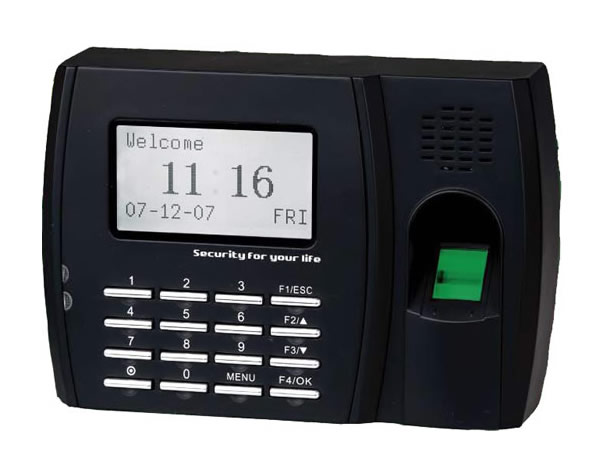
\includegraphics[scale=0.4]{fingerprint_u300.png}
 \end{center}
 \caption{Lector de huellas digitales U300 de ZKSoftware}
 \label{fig:finger_print_7}
\end{figure}

Una de las principales características de este lector, es que una vez configurada su dirección IP, se puede acceder a una página web para consultar los registros almacenados. Se pueden obtener registros del día actual, de ayer, de la semana pasada, o bien especificar la fecha para desplegarlos. 

\begin{figure}[htb]
 \begin{center}
  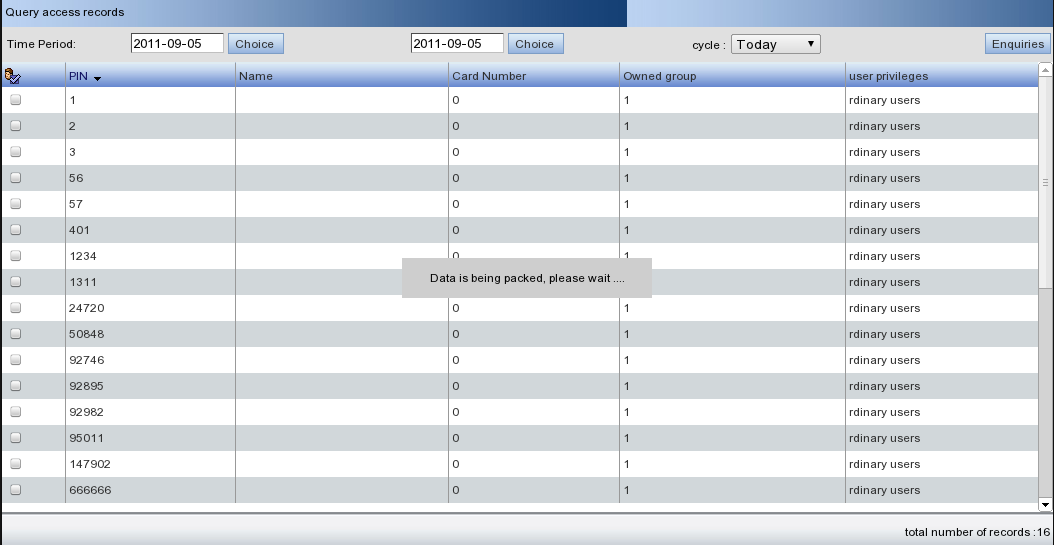
\includegraphics[scale=0.4]{fingerprint_web_2.png}
 \end{center}
 \caption{Página web del dispositivo mostrando usuarios registrados.}
 \label{fig:finger_print_8}
\end{figure}

En la figura \ref{fig:finger_print_8} se observa la página para seleccionar los usuarios almacenados en el lector y poder consultar sus registros de acuerdo a la fecha indicada. El procedimiento para obtener los datos y el registro de los empleados es el siguiente:

\begin{enumerate}
 \item Mediante cURL\footnote{cURL es una herramienta para usar en un intérprete de comandos para transferir archivos con sintaxis URL, soporta FTP, FTPS, HTTP, HTTPS, TFTP, SCP, SFTP, Telnet, DICT, FILE y LDAP.} se debe obtener la cookie de la página web del lector de huellas digitales, para poder consultar los registros.
 \item Con la cookie previamente descargada y con cURL se accede a la dirección \url{http://192.168.101.23/form/AttLog}. En este caso la IP del lector de huellas es \texttt{192.168.101.23}. Con esto se obtiene la imagen de la figura \ref{fig:finger_print_8} que sirve para obtener los números de empleados de los usuarios registrados.
 \item Con cada uno de los números de empleados obtenidos en el punto anterior, se consulta con cURL el URL \url{http://192.168.101.23/form/AttLog?act=1} con la fecha indicada, con lo que se obtiene la página con los registros almacendados para ese usuario. En caso de que el usuario no tenga registros para ese día, se pasa al siguiente usuario.
 
 \begin{figure}[htb]
 \begin{center}
  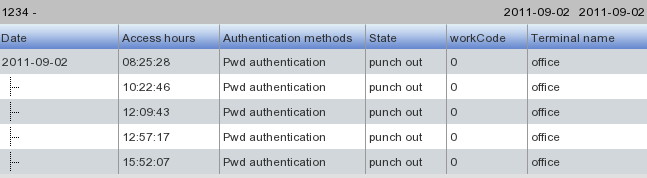
\includegraphics[scale=0.6]{fingerprint_web_3.png}
 \end{center}
 \caption{Página web mostrando los registros de un usuario.}
 \label{fig:finger_print_9}
\end{figure}
 
 \item Con ayuda de Perl y el módulo \texttt{HTML::TableExtract} se parsea la página HTML obtenida en el punto anterior y se obtiene principalmente, la columna de hora. Se parsean todas los renglones de hora que existan. Por lo menos debe existir un registro de hora, la cual se considera la entrada. El último registro se considera la salida, en caso de que existan más de 2 horas registradas.
 \item Con el ID del usuario, la fecha y la hora de entrada y/o salida, se realiza una consulta a la base de datos de PostgreSQL para revisar si no ha habido registro de este usuario.
 \begin{itemize}
  \item Si tiene un registro de hora, es su entrada, se registra en base de datos y en los archivos necesarios en el punto de venta.
  \item Si tiene dos registros de hora, es su salida, y se registra en la tabla de la base de datos y se actualizan los archivos correspondientes del punto de venta.
  \item Si tiene más de dos registros, se toma el último registro de hora, para la salida, en este caso se actualiza el valor en la tabla de salida y en los archivos correspondientes del sistema punto de venta.
 \end{itemize}

\end{enumerate}

Este proceso se lleva a cabo en un proceso CRON cada minuto. Lo que garantiza que una vez que el usuario ha realizado su verificación en el lector, éste pueda utilizar de manera casi inmediata el sistema punto de venta.  No todos los usuarios utilizan directamente las terminales, el único puesto que maneja directamente las terminales son las personas que atienden los destinos de servicio a domicilio y auto (este destino es aquel en que el cliente ingresa con su carro al estacionamiento y realiza la orden desde él); por lo que se ejecute cada minuto el proceso que lee y procesa los datos del lector es correcto para la operación.

A la fecha el desarrollo ya se encuentra funcionando al 100\% y en prueba en dos restaurantes, no se ha liberado a más centros debido a que el área de Operaciones y Legal debe realizar adecuaciones a los contratos actuales, así como la de elaborar un plan de entrenamiento a los empleados.

Es muy importante que en el momento del enrolamiento o la verificación se coloque de manera adecuada el dedo, ya que de otra manera, existirán errores de captura/lectura. La correcta forma de colocar el dedo en el centro del lector de una manera plana y firme.

\begin{figure}[htb]
 \begin{center}
  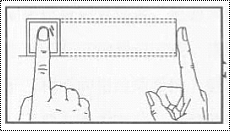
\includegraphics[scale=0.7]{place_finger_1.png}
 \end{center}
 \caption{Forma ideal para colocar el dedo en el lector.}
 \label{fig:finger_print_10}
\end{figure}

Es considerada una mala colocación del dedo en el lector, cuando el dedo no se encuentra completamente plano, no se encuentra en el centro del lector, ya sea que esté muy a la derecha, izquierda o abajo. O cuando el dedo no haga contacto la huella digital con el lector.

\begin{figure}[htb]
 \begin{center}
  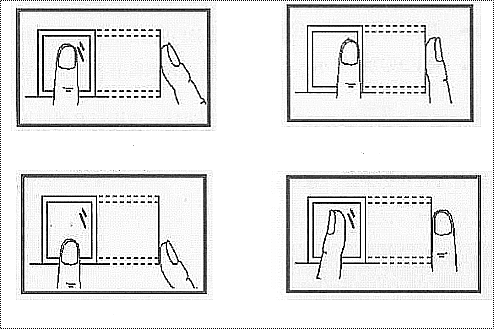
\includegraphics[scale=0.7]{place_finger_2.png}
 \end{center}
 \caption{Forma incorrectas para colocar el dedo en el lector.}
 \label{fig:finger_print_11}
\end{figure}